\lecture{Thu. 9/13/12}

Last time we talked about 
\begin{itemize}
\item
nondeterminism and NFA's
\item
NFA$\to $DFA
\item
Regular expression$\to$ NFA
\end{itemize}
Today we'll talk about
\begin{itemize}
\item
DFA$\to $regular expression
\item
Non-regular languages
%\item Context-free grammars.
\end{itemize}
%recitations start tomorrow F11, F12, 2-143, optional unless having problems.

%hw: try over a week in advance.s
About the homework: By the end of today, you should have everything you need to solve all the homework problems except problem 6. Problem 3 (1.45) has a 1 line answer. As a hint, it's easier to show there {\it exists} a finite automaton; you don't have to give a procedure to construct it.


We will finish our discussion of finite automata today. We introduced deterministic and nondeterministic automata. Nondeterminism is a theme throughout the course, so get used to it.

We gave a procedure---the subset construction---to convert NFA to DFA. NFA helped achieve part of our goal to show regular expressions and NFAs recognize the same languages. We showed how to convert regular expressions to NFA, and NFA can be converted to DFA. To convert regular expressions, we used the constructions for closure under $\cup$, $\circ$, and ${}^*$; we start with the atoms of the expression, and build up using more and more complex subexpressions, until we get the language recognized by the whole expression. This is a recursive construction, i.e. a proof by induction, a %Two words for the same thing. 
proof that calls on itself on smaller values.

Today we'll do the reverse, showing how to convert a DFA to a regular expressions, finishing our goal.
\subsection{Converting a DFA to a regular expression}
\begin{thm}[Theorem~\ref{thm:regex-FA}, again]
$A$ is a regular language iff $A=L(r)$ for some regular expression $r$.
\end{thm}
%iff have to prove 2 directions
\begin{proof}
$\Leftarrow$: Show how to convert $r$ to an equivalent NFA. We did this last time.

$\Rightarrow$: We need to convert a DFA to an equivalent $r$. This is harder, and will be the focus of this section. %Simulating expression with automata is more natural, like programming.
\end{proof}
We'll digress and introduce another model of an automaton, which is useful just for the purposes of this proof.

A \textbf{generalized nondeterministic finite automaton (GNFA)} has states, some accepting, one of which is starting. We have transitions as well. What's different is that we can write not just members of the alphabet and the empty string but any regular expression as a lable for a transition. So for instance we could write $ab$.

\begin{center}
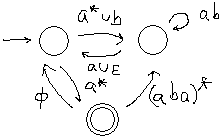
\includegraphics{3-1}
\end{center}

Start at the start state. During a transition, the machine gets to read an entire chunk of the input in a single step, provided that the string is in the language described by the label on the associated transition.

There may be several ways to process the input string. The machine accepts if some possibility ends up at an accept state, i.e. there is some way to cut and read the input string. If all paths fail then the machine rejects the input.

Although GNFA's look more complicated, they {\it still recognize the same languages as DFA's!}

If looks harder to convert a GNFA to a regular expression,  GNFA$\to$r. However, for inductive proofs, %Recursive proofs by induction: H
it is often helpful to prove something stronger along the way, so we can carry through the statement. In other words, we {\it strengthen} the induction hypothesis.

To make life easier, we make a few assumptions about the GNFA.
\begin{itemize}
\item
First, there is only 1 accept state. To achieve this, we can declassify accept states, and add empty transitions to new accept states. 
\item The accept state and start states are different (taken care of by 1st bullet).
\item No incoming transitions come to the start state. To achieve this, make a new start state with an $\ep$-transition going to the previous start state.
\item There are only transitions to, not from, the accept state (taken care of by 1st bullet).
\item Add all possible transitions between states except the start and end states. If we are lacking a transition, add $\phi$ transition. We can go along this transition by reading a language described by $\phi$. This means we can never go along this transition, since $\phi$ describes no languages.
%\item There is only one transition from a state $i$ to a state $j$. To achive this, take the union of all languages on arrows from $i$ to $j$.
\end{itemize}

For instance, we can modify our example to satisfy these conditions as follows.

\begin{center}
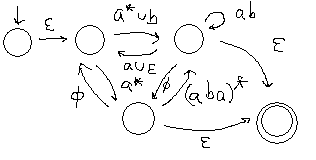
\includegraphics{3-2}
\end{center}

\begin{lem}
For every $k\ge 2$, every GNFA with $k$ states has an equivalent regular expression $R$.
\end{lem}
\begin{proof}
We induct on $k$. 

The base case is $k=2$. We know what the states are: the machine has a start state (no incoming arrows) and an accept state. Assuming the conditions above, the only possible arrow is from the start to end, so the machine looks like the following. There are no return arrows or self-loops.

\tikzstyle{state}=[circle,draw,inner sep=0pt,minimum size=6mm]
\tikzstyle{accept}=[circle,draw,inner sep=0pt,minimum size=7.5mm]
\begin{center}
\begin{tikzpicture}[->,>=stealth',shorten >=1pt,auto,node distance=1cm,semithick]
\node (0) at (-1,0) {};
\node (1) at ( 0,0) [state] {$q_1$};
\node (2) at ( 2,0) [state] {$q_2$};
\node (2) at ( 2,0) [accept] {$q_2$};
\draw (0) edge node {} (1);
\draw (1) edge node {$R$} (2);
\end{tikzpicture}
\end{center}

The only way to accept is to read a string in $R$; the machine can only process input in its entirety with one bite, so the language is just the regular expression $R$. This is the easy part.

Now for the induction step. Assume the lemma true for $k$; we prove it for $k+1$. Suppose we're given a $(k+1)$-state GNFA. We need to show this has a corresponding regular expression. We know how to convert $k$-state GNFA to a regular expression. Thus, {\it if we can convert the $(k+1)$-state to a $k$-state GNFA,  then we're done.} You can think of this as an iterative process: convert $(k+1)$ to $k$ to $k-1$ states and so on, wiping out state after state, and keeping the language the same, until we get to just 2 states, where we can read off the regular expression from the single arrow. 

We'll pick one state $x$ (that is not the start or accept state) and remove it. Since $k+1\ge 3$, there is a state other than the start and accept state. But now the machine doesn't recognize the same language anymore. We broke the machine! 

\begin{center}
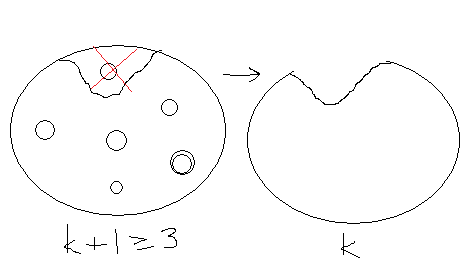
\includegraphics[scale=0.5]{3-4}
\end{center}

We have to repair the machine, by putting back the computation paths that got lost by removing the state.

This is where the magic of regular expressions come in.

Suppose we have arrows $i\to x\to j$. We can't follow this path because $x$ is gone. In the arrow from $i$ to $j$, we have to put back the strings that got lost. So if we have $i\xra{r_1}x\xra{r_3} j$, then we add in $r_1r_3$ from $i$ to $j$, so we can go directly from $i$ to $j$ via $r_1r_3$. %Now take the union with the regular expression from $i$ to $j$, $r_1r_3\cup r_4$. But there might be a self loop on $x$, say $r_2$.
However, letting the self-loop at $x$ be $r_2$, we might go along $r_1$, repeat $r_2$ for a while, and then go to $r_3$, we so actually want $r_1(r_2^*)r_3$. Now take the union with the regular expression from $i$ to $j$, $r_1(r_2^*)r_3\cup r_4$.

\begin{center}
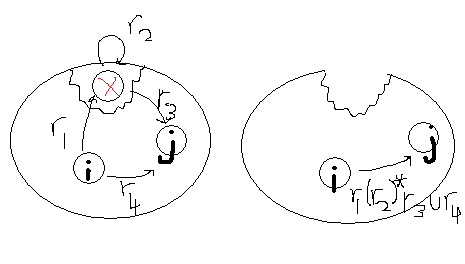
\includegraphics[scale=0.5]{3-5}
\end{center}

So the construction is as follows. For each pair $i\xra{r_4} j$, replace  $r_4$ with
\[
r_1(r_2)^*r_3\cup r_4
\]
where $r_1$, $r_2$, $r_3$ are as above.
All arrows adjusted in the same way. The computations that go from $i$ to $j$ via $x$ in the old machine are still present in the new machine, and go directly from $i$ to $j$. 

%For every pair of states, every transition, change the label in the new machine so get the same effect go from i to j as i to x to j.
Our modified machine is equivalent to the original machine. Taking any computation in first machine, there is a corresponding computation in second machine %mirrors in first machine 
on the same input string, and vice versa. This finishes the proof. %i to x to j, captured in new machine. Recover i to x to l to x to j. i to x to l got modified, captured in transition that goes from i to l. Only need to deal with case from state to removed case (sit for awhile) to another state. Don't need more complicated routes than that
%computation die at x. Don't need add anything!

%We haven't added anything either. Haven't lost: take computation go through x. Look all runs, take states bordering run, go directly from i to j in RHS. 
\end{proof}
%how big/efficient are conversions?
%last time: about the same size. linear size (const factor larger
%DFA to r, horrendously larger. do example with 5 states. Do on every transition. roughly 4 times bigger. Every time remove another state, multiply by 4. Get big fast. Neither direction optimal, this optimal. 
%smallish NFA, large DFA. (Power set, exponential increase)
Theorem~\ref{thm:regex-FA} now follows, since a DFA is a GNFA.
\subsection{Non-regular languages}
There are lots of langages that are not recognized by any finite automata. We see how to prove a specific language is non-regular.

Let 
\[
C=\set{w}{w\text{ has equal number of 0s and 1s}}.
\]
As we've said, it seems like $C$ is not regular because it has to keep track of the difference between the number of 0s and 1s, and that would require infinitely many states. But be careful when you claim a machine can't do something---maybe the machine just can't do it the following the method you came up with! \\


\wrbox{``I can't think of a way; if I try come up with one I fail" doesn't hold water as a proof!}
%Different but capabilities within the machine.
\vskip0.15in
As an example, consider %Something looks superficially like need to account, but alternative avoid need to count. For example
\[
B=\set{w}{w\text{ has equal number of 01 and 10 substrings}}.
\]
For example $1010\nin B$, but $101101\in B$. This language may look nonregular because it looks like we have to count. But it is regular, because there is an alternative way to describe it that avoids counting.\\

\prbbox{Show that $B$ is regular.}
\vskip0.15in
\subsubsection{Pumping Lemma}
We give a general method that works in large number of cases showing a language is not regular, called the Pumping Lemma. It is a formal method for proving nonregular not regular. Later on, we will see similar methods for proving that problems cannot be solved by other kinds of machines.


\begin{lem}[Pumping Lemma]\llabel{lem:pump}
For any regular language $A$, there is a number $p$ where if $s\in A$ and $|S|\ge p$ then $S=xyz$ where
\begin{enumerate}
\item 
$xy^iz\in A$ for any $i\ge 0$ (We can repeat the middle and stay in the language.)
\item
$y\ne \ep$ (Condition 1 is nontrivial.)
\item
$|xy|\le p$ (Useful for applications.)
\end{enumerate}
\end{lem}
What is this doing for us? The Pumping Lemma gives a property of regular languages. To show a language is not regular, we just need to show it doesn't have the property.

The property is that the language has a {\it pumping length}, or cutoff $p$. For any string $s$ longer than the cutoff, we can repeat some middle piece ($y^i$) as much as we want and stay in the language.  We call this {\it pumping up} $s$. %Take middle part, pump $s$, get bigger and bigger. Like bicycle tires. 
Every long enough string in the regular language can be pumped up as much as we want and the string remains in the language. 

Before we give a proof, let's see an example.
\begin{ex}
Let 
\[D=\set{0^m1^m}{m\ge 0}.\] Show that $D$ is not regular using the Pumping Lemma. \\

\cpbox{
To show a language $D$ is not regular, proceed by contradiction: If $D$ is regular, then it must have the pumping property. Exhibit a string of $D$ that cannot be pumped no matter how we cut it up. This shows $D$ does not have the pumping property, so it can't be regular.}
\vskip0.15in
Assume $D$ is regular. The pumping lemma gives a pumping length $p$. We find a string longer than $p$ that can't be pumped: let $s=0^p1^p\in D$.

\begin{center}
\includegraphics{diagrams/diags-4}
\end{center}

There must be some way to divide $s$ into 3 pieces, so that if we repeat $y$ we stay in the same language.

But we can't pump $s$ no matter where $y$ is. One of the following cases holds:
\begin{enumerate}
\item
$y$ is all 0's
\item
$y$ is all 1's
\item
$y$ has both 0's and 1's.
\end{enumerate}•
If $y$ is all 0's, then repeating $y$ gives too many 0's, and takes us out of the language. If $y$ is all 1's, repeating gives too many 1's. If $y$ has both 0's and 1's, they are out of order when we repeat. In each case, we are taken out of the language so pumping lemma fails, and $D$ is not regular.

%Cases where $y$ lives when cut off. In each case, take out of language so pumping lemma fails. 
If we use condition 3 of the Pumping Lemma we get a simpler proof: $xy$ is entirely in the first half of $s$, so $y$ must be all 0's (case 1). Then $xyyz$ has excess 0's and so $xy^2z\nin D$.
\end{ex}

Now we prove the Pumping Lemma.
\begin{proof}[Proof of Lemma~\ref{lem:pump}]
Let $M$ be the DFA for $A$. Let $p$ be the number of states of $M$. This will be our pumping length. %some state repeat!

Suppose we have a string of length at least $p$. 
Something special has to happen when the machine reads the string: {\it We have to repeat a state!} %(Because we start at a state at step 0, we have to make at least $p+1$ visits to state.)
%More symbols than state, because starting before first. 
%There has to be a repeated state. 
We have to repeat a state within the first $p$ steps (because after $p$ steps we've made $p+1$ visits to states, including the starting state). Consider the first repeated state, drawn in in the below diagram.

\begin{center}
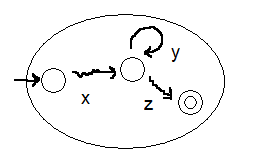
\includegraphics{3-6}
\end{center}

Divide the path into 3 parts: $x$, $y$, and $z$. %pumpable.
%pump down by removing y.
Note we can choose $y$ nonempty because we're saying the state is repeated. %(3) is true because we choose the first time it repeats.
From this we see that we can repeat $y$ as many times as we want.
\end{proof}
\begin{ex}
Now we show 
\[
C=\set{w}{w\text{ has equal number of 0s and 1s}}.
\]
is not regular. There are two ways to proceed. One is to use the Pumping Lemma directly (this time we need to use condition $3$) and the other way is to use the fact that we already know $D$ is not regular.

What is wrong with the following proof? Because $D$ is not regular and $D\subeq C$, $C$ is not regular.\\

\wrbox{
Regular languages can have nonregular languages as subsets, and vice versa. Subsets tell you nothing about regularity.
} 
\vskip0.15in
However, we if we combine the fact that $D\subeq C$ with some extra features of $C$, then we can come up with a proof. Note
\[D=C\cap 0^*1^*.\]
Note $0^*1^*$ is regular. If $C$ were regular, then $D$ would be regular, because the intersection of 2 regular languages is regular. Since $D$ is not regular, neither is $C$.\\

\cpbox{
The Pumping Lemma is a powerful tool for showing languages are nonregular, especially when we combine it with the observation that regular languages are closed under regular operations.
}

\end{ex}